\begin{frame}[c]
  \frametitle{Case IV : Partition Coefficient}
The retardation factor, $R_f$, which is the ratio between velocity of water through a 
volume and the velocity of a contaminant through that volume, can be expressed 
in terms of the partition coefficient,

\begin{align}
  R_f &= 1+\frac{\rho_b}{n_e}K_d
  \intertext{where}
  \rho_b &= ~~\mbox{bulk density}[kg\cdot m^{-3}]\nonumber
  \intertext{and}
  n_e &= ~~\mbox{effective porosity of the medium}[\%].\nonumber
\end{align}
The coefficient $K_d$, in units of $[m^3\cdot kg^{-1}]$, is the ratio of the mass of contaminant in the solid to the mass of contaminant in the solution.
\end{frame}

\begin{frame}[c]
  \frametitle{Case IV : Partition Coefficient}

The parameters in this model were all set to the default values except a multiplier 
applied to the partitioning $K_d$ coefficients.
\begin{table}[ht!]
\centering
\footnotesize{
\begin{tabular}{|l|l|l|r|r|}
\multicolumn{5}{c}{\textbf{Simulation Cases}}\\
\hline
\textbf{Case} & \textbf{Parameter} & \textbf{Units} & \textbf{Min. Value} & \textbf{Max. Value}\\
\hline
IV    & $K_{d,i}$    & $[m^3\cdot kg^{-1}]$       & $(1\times10^{-9})\langle K_{d,i}\rangle $    &  $(5\times10^{10})\langle K_{d,i}\rangle $ \\
\hline
\end{tabular}
\caption{Case IV varied the partitioning coefficient, $K_d$, multiplication 
  factor. This single parameter simulation case had 40 simulation 
groups of 100 realizations each.}
\label{tab:Cases}
}
\end{table}


\end{frame}

\begin{frame}[c]
  \frametitle{Case IV : Partition Coefficient}

\begin{figure}[ht]
\centering
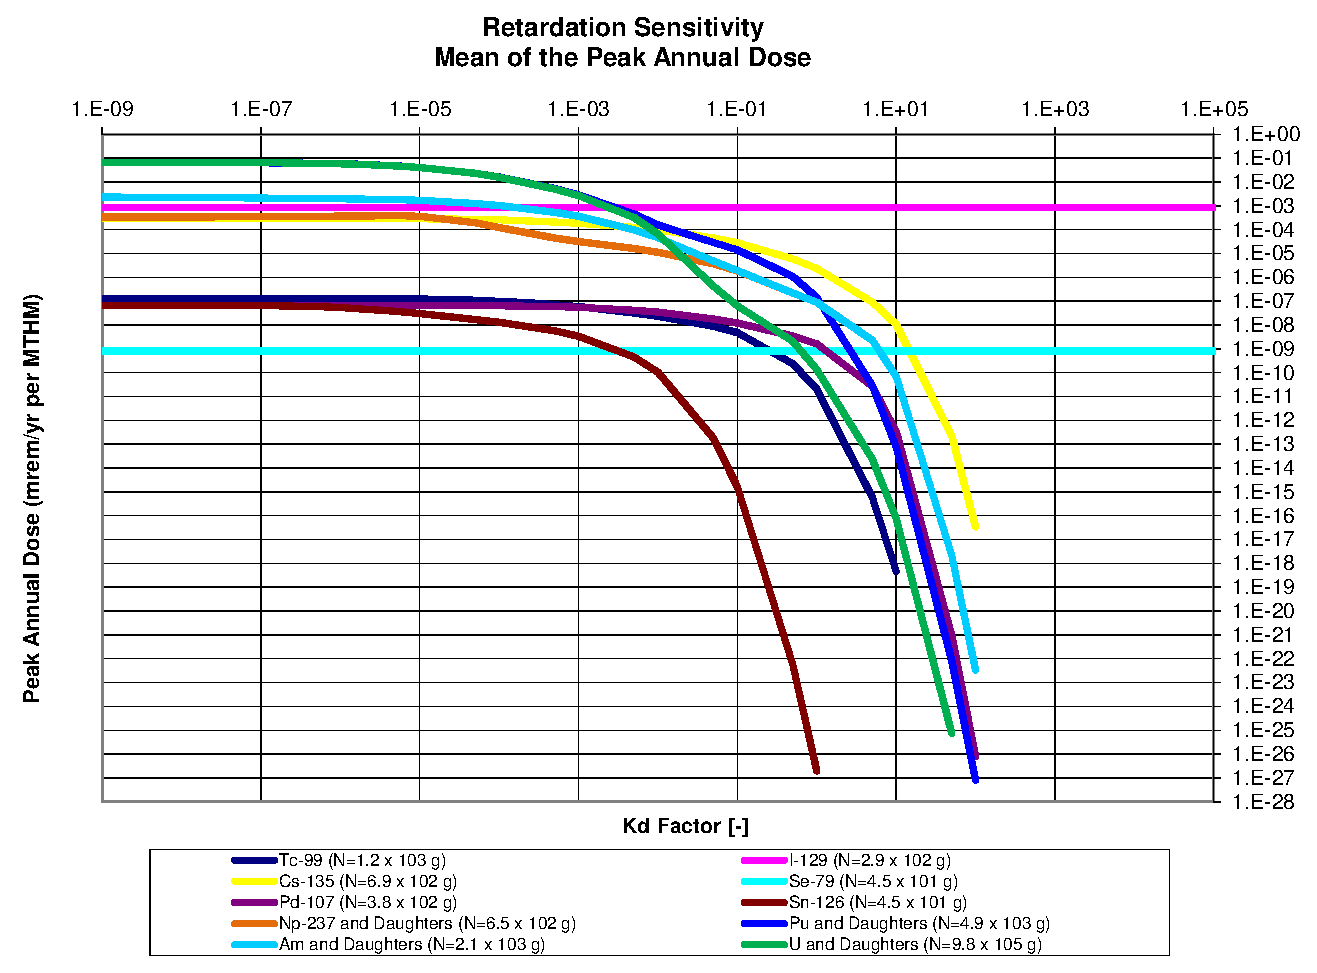
\includegraphics[width=0.8\textwidth]{Sorption/Retardation_Summary_kdFactor.eps}
\caption{
For retardation coefficients greater than a threshold, the 
relationship between peak annual dose and retardation coefficient is a strong 
inverse one. }
\label{fig:KdSumFactor}
\end{figure}
\end{frame}

\begin{frame}[c]
  \frametitle{Case IV : Partition Coefficient}

\begin{figure}[ht]
\centering
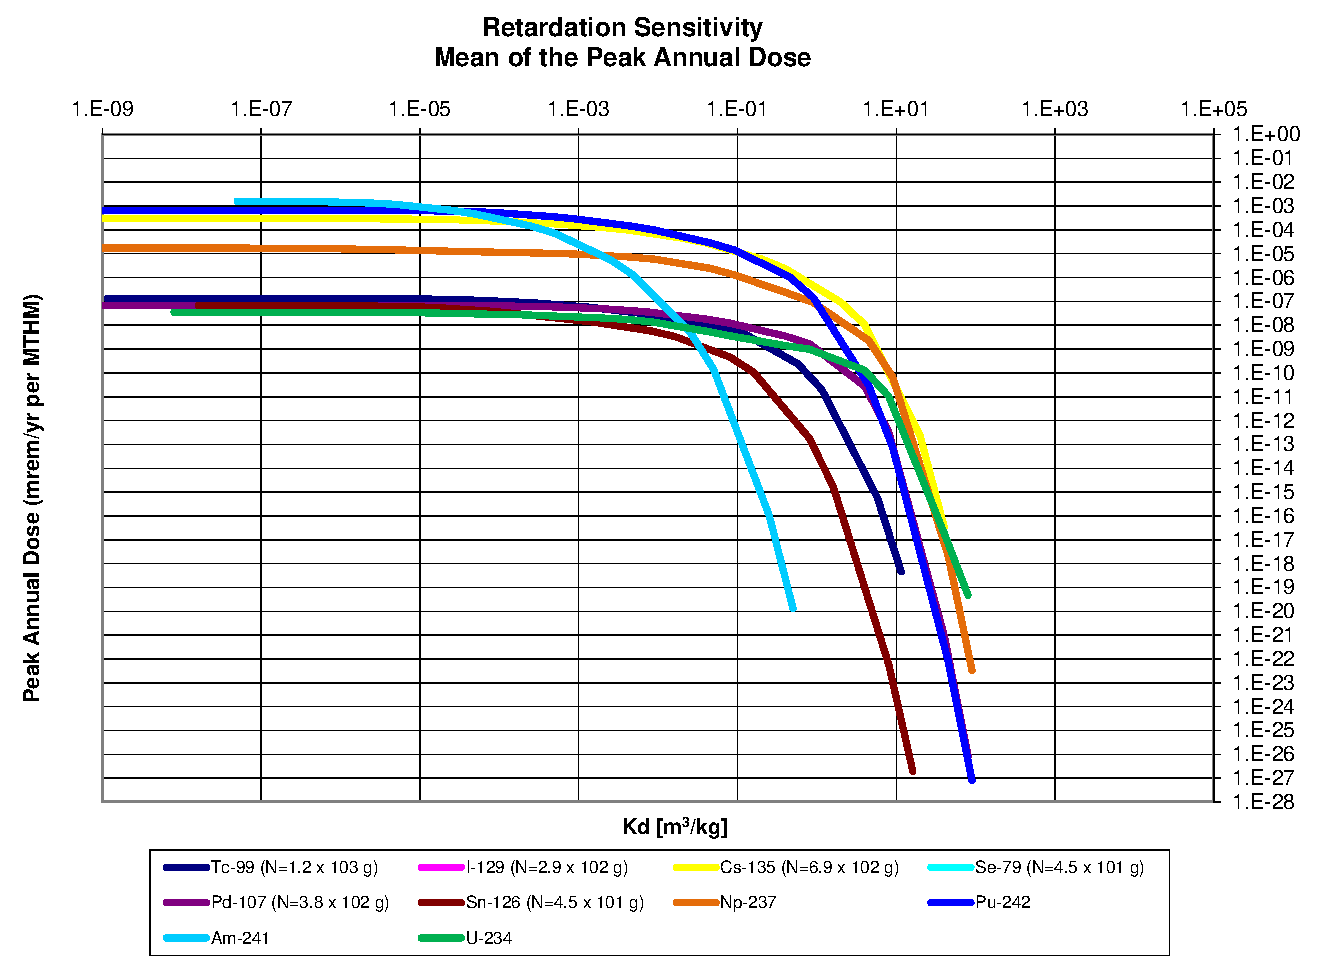
\includegraphics[width=0.8\textwidth]{Sorption/Retardation_Summary_kd.eps}
\caption{
For retardation coefficients greater than a threshold, the 
relationship between peak annual dose and retardation coefficient is a strong 
inverse one. }
\label{fig:KdSum}
\end{figure}
\end{frame}

